\documentclass[a4paper]{article}
\usepackage[english]{babel}
%\usepackage[utf8x]{inputenc}
\usepackage{amsmath}
\usepackage{amssymb}\usepackage{graphicx}
\usepackage{multicol}
\usepackage{float}
\usepackage{textcomp}
\usepackage{gensymb}
\usepackage{listings}
\usepackage{color}
\usepackage[margin=1cm]{caption}
\usepackage[margin=1in]{geometry}
\usepackage{fancyhdr}

\title{Debris-Informed Underwater Search and Rescue Optimized in Two Parts}
\author{}
\date{}

\newcommand*{\Scale}[2][4]{\scalebox{#1}{$#2$}}
\pagestyle{fancy}
\fancyhf{}
\lhead{Team 40670}
\rhead{Page \thepage\, of ***}

\definecolor{dkgreen}{rgb}{0,0.6,0}
\definecolor{gray}{rgb}{0.5,0.5,0.5}
\definecolor{mauve}{rgb}{0.58,0,0.82}
\definecolor{black}{rgb}{0,0,0}

\renewcommand\thesection{\arabic{section}}
\renewcommand\thesubsection{\thesection.\arabic{subsection}}
\renewcommand\thesubsubsection{\thesubsection.\arabic{subsubsection}}

%\setlength\parindent{0em}
%\setlength{\parskip}{5pt}
%\renewcommand{\theenumi}{\Alph{enumi}}
\begin{document}\maketitle

\begin{abstract}
A model for optimal discrete-effort search for a plane lost in open ocean is presented. A pre-existing ocean current model is assumed to generate probability distributions for debris and the plane body in the search area. The search region is split into smaller cells. An aerial search is then executed for debris. The probability distribution for the location of the plane body on the seafloor is then modified by the current model using a statistical transformation on the data. Searches underwater are then optimized with respect to chance of discovery and search cost. Two search cost functions are compared. Both searches are generalized with respect to the search technology used. A measure of the efficiency of search technologies is referenced and assumed to be given by other research. In this way, the model is generalized with respect to search technology used; any technology will work. Results of test runs demonstrate a logarithmic relationship between percent success and both quantity of search vehicles as well as quantity of searches. The computational cost of the model is estimated at $O(n)$ with respect to both quantity of search iterations and quantity of search vehicles. A comparison is made between a simulation that optimizes cost, which is expressed as a function of total search vehicle travel distance, and one that does not. This comparison revealed that optimizing the travel distance may reduce total distance traveled by up to a factor of 38 while only marginally sacrificing total search effectiveness.
\end{abstract}

\pagebreak 

\section{Introduction}

The expansion of air travel will lead to the occasional and inevitable ocean plane crash. In order to maximize the chance of successful recovery, it is important to have a working model on-hand for how to best execute such a search. 

This paper contains a discussion of an optimal search for a missing object based on a probabalistic distribution. It has been generalized to the point where any available search technology may be included, and any type of craft may be sought.

However, specific technologies are not modeled in this paper. It is assumed that, through other research and testing, relatively accurate models for the detection rate of the search technologies used have been acquired. Additionally, it is presupposed that a model exists for current that will allow for both backward and forward tracking. Existing research suggests such a model exists.

As a result, three abstractions have been achieved. First, an abstraction with respect to the physical search space: the current model(s) return a probability distribution for debris across the surface of the water and for the position of the craft on the sea floor. 

Secondly, there is an abstraction with respect to the search technology used: the detection rate of this technology in locating an object is given by research using that specific technology. Specific search technologies are not included in this paper for two reasons: the state of the art advances quickly, and rigorous testing with equipment is needed to determine these values. 

Thirdly, there is an abstraction with respect to the type of fallen plane. This is done in the same way as the abstraction with respect to search technology. This abstraction is, in this context, the percent chance that a search technology will detect a particular object. The chance will change with both the object type and the search technology used.

\section{General Discrete-effort Optimal Searching}

A modified discrete-effort method derived Lawrence Stone's \textit{Theory of Optimal Search} is used in both searches to prioritize and distribute search efforts. An overview of this method is provided here. 

\subsection{Defining the Terms Used in Searching}

The search space $\mathcal{J}$ is divided into an integer number of uniformly square cells $j\in\mathcal{J}$. The specific technologies (i.e. one type of Autonomous Underwater Vehicle versus another) used in the search are indexed for convenience by integers in $\mathcal{T}$. This allows for implementation of different measurement accuracies and cost functions as search technology advances, or simply as different technology is chosen. 

For each search technology $t\in\mathcal{T}$ used, each cell $j\in\mathcal{J}$ is associated with a cost of searching. This cost is expressed in terms of the cell number and the number of times searched: $\gamma_t(j,k)$. This represents the cost of the $k$th search in cell $j$ using technology $t$.

It is important to note that $\gamma_t(j,k)$ can be defined with respect to a general cost function, $c_t(j,k)$; by contrast, $c_t$ is the cost of searching  a \textit{total} of $k$ discrete times. Ergo, $$\gamma_t(j,k_n)=c_t(j,k_n)-c_t(j,k_{n-1})$$

The probability of debris existing in a given cell is denoted by $p(j)$.

Finally, $\beta_t(j,k)$ is the probability of locating an object in cell $j$ using tech $t$ on the $k$th attempt, assuming that the object is actually in cell $j$.

The quantity $p(j)\beta(j,k)$ represents the actual chance of finding debris in the $j$th cell on the $k^{th}$ search. $\beta$ assumes the object is in the current cell being searched, where the product $\beta * p$ does not assume so.

Next, the optimization problem is stated. The optimal individual cell to focus the search methods on is the one which provides the highest chance of success per unit search cost. This value, denoted as $\epsilon$, is defined as $$\epsilon_t\equiv\epsilon_t(j,k)=\frac{p(j)\beta_t(j,k)}{\gamma_t(j,k)}$$. 

An $\epsilon$ can be computed for each cell, accounting for the number of searches $k$ for each one. The highest values are the ones with the greatest probability of success per unit cost. 

\subsection{Assigning Values to $\beta_t(j,k)$}

Suppose $\alpha_t$ is the success rate for locating an object, whether underwater or aerial, with $t\in\mathcal{T}$. Then, from \textit{Theory of Optimal Search}: \[\beta_t(j,k)=\alpha_t\cdot(1-\alpha_t)^{k-1}\]

This representation follows that each successive search has an exponentially decreasing chance of success. The derivation is not copied here. It is worth noting, however, that the $\alpha_t$ value will significantly depend on the technology used and the context within the model is applied.

\subsection{Cost Functions as Prioritization}

The cost $\gamma_t(j,k)$ provides flexibility for the model in terms of prioritization. Considerations such as distance, time, and money may be confounding variables in the cost of searching. The resulting function $\gamma$ will depend entirely on the technology being used. In this model, the cost of searching a cell is assumed to be equal to the distance traveled to reach the cell. In this way, distance, travel time, and monetary cost are roughly minimized.

In this model, the distance parameter in the cost of the function, such that $\gamma_t(j,k)=d_{travel}$, where $d_{travel}$ is the Euclidean distance in cells from the current position to the position under consideration. This has the benefit of moving ships around as little as possible. One may extend the cost function by including the time to search - in other words, $\gamma(j,k)=t_{search}+d_{travel}$. The inclusion of travel time implies specifying the technology to be used, however; as a result, this method of prioritization is not included here.  

\subsection{Evolving Probability Distributions over Failed Searches}

In the event that the model does not find an object in cell $k$, the probability distribution must be modified to accommodate for the altered search area. Let $T$ represent the probability that the plane is in the cell, and $F$ the probability that it is found. Then: 
$$P(T|F)=\frac{P(T)P(F|T)}{P(F)}$$ 
$$P(T|\sim F)=\frac{p(j)[1-\beta_t(j,k)]}{(p(j)[1-\beta_t(j,k)]+(1-p(j))}$$

By reduction, the posterior probability that the object is there but was not found is: $$p'(j)=p(j)\frac{1-\beta_t(j,k)}{1-\beta_t(j,k)p(j)},\;\mbox{where }j\mbox{ is searched}$$.

The posterior probability of every other square can be similarly adjusted by the knowledge that an object was not discovered in cell $k$ (though its proof is omitted): $$p'(j)=p(j)\frac{1}{1-p(j)\beta_t(j,k)},\;\mbox{where }j\mbox{ is not searched.}$$

After the application of these transformations, as $p'$ is a probability distribution, the quantity $$\sum_{j\in\mathcal{J}}p'(j) = 1$$

(The notation here may be confusing. For clarification, the first $p'(j)$ adjustment applies only to the square that was searched; the second applies to every other square.)

After a failed search, the probability of the plane being in cell $j$ becomes this probability.

\subsection{Executing the Search Method}

Suppose there is a set $\mathcal{T}$ of search technologies and $n_t$ instances of technology $t\in\mathcal{T}$. For each device, the $\epsilon$ value is computed. Optimizing this value returns the highest probability of object discovery per unit cost.

Each device is allocated sequentially to a square that is a) not already being searched, and b) has the highest $\epsilon$ value for that technology. Should two devices conflict in their optimal square, the closest device of that type claims it. Though travel time is not modeled, it is reasonable to make preliminary decisions in deference to it.

Whenever a device finishes searching, the probability distribution of the object's position is recomputed according to the above transformation, the device's $\epsilon$ value is recomputed based on the new distribution, and it is assigned to a new cell.

The net success is the cumulative product of $p_t(j)*\beta_t(j,k)$. Suppose $f_t(j)$ is the total number of searches allocated to cell $j$. Then, the net probability that the plane has been discovered by a single technology can thus be expressed as: $$\sum p_t(j)\beta_t(j,f_t(j))$$

\section{Assumptions}

Assumptions may be broken into three categories: general assumptions, assumptions used for the aerial search, and assumptions used for the underwater search. A note that an assumption ``is extensible'' is used to indicate that the removal of the assumption from the model does not significantly complicate the mathematics used.

While many of these assumptions can be removed from the model, the actual process for doing so is typically not included in this paper; however, an overview is given for all extensible assumptions.

\subsection{General Assumptions}

\begin{itemize}
\item A known search space already exists between departure point and destination point.
\item Only one search occurs in a cell at a time; only one vessel occupies a cell at a given time. This assumption is extensible by programmatically allowing multiple vessels to be in a given cell. However, the process for computing the probability of success is complicated by this extension, and is excluded from this paper.
\item When computing distances, the curvature of the Earth is ignored; each cell size is considered small enough to approximate Euclidean distance. This is done to simplify the consideration of a two-dimensional grid; extension is fully possible through the inclusion of a concrete distance.
  
\item It is assumed that the time between issuing a search instruction and the time until that search begins is approximated by the distance the vessel has to move. This assumption is only partially extensible; inclusion of time into the model requires reworking the $\gamma$ function to vary with both distance and time.
\item All cells are of equal size. This is relatively extensible. In order to adjust for this, however, one would need to adjust the probability of success, the cost of searching, and the probability of the object being in the cell according to the area of the cell. This is not a simple process, and it is not included here.
\end{itemize}

\subsection{Aerial Search Assumptions}

\begin{itemize}
\item An accurate model regarding ocean currents' ability to shift objects exists that is suitable for use in conjunction with this model. Such a current model needs to advance in either continuous-time or small discrete-time steps, as the probability distribution of debris will change vastly both over time and number of searches. Previous research suggests such a model exists. 
\item Debris is either present or not present. Various types of debris and their individual implications are not considered. 
\end{itemize}

\subsection{Underwater Search Assumptions}

\begin{itemize}
\item Unlimited iterations of searching are allowed. While it would be possible to allow for finite searching without changing the algorithm, the search algorithm, as-is, would no longer be optimal. 
After all available effort has been allocated, the algorithm would need to provide a best-guess answer. Hence, a constraint on effort allocation places an additional constraint on optimization.  This modification constitutes a significant mathematical change.
\item A current model exists that can predict an initial probability distribution of the position of the plane body on the sea floor. This probability distribution will be later informed by discovered debris.
\item The plane does not drift once it makes contact with the sea floor.  
\item The success of a vehicle searching a space can be measured directly as a probability of success, regardless of surroundings and extenuating conditions. This assumption also implies that either the sea floor is of uniform depth and topography, or that the depth and topography of the sea floor is not relevant to plane discovery. While this is likely a weak assumption, this \textit{it} extensible simply by making the $\beta_t(j,k)$ function vary with cell $j$ as a function of sea floor depth. 
\end{itemize}

\section{Current Flow Modeling and Aerial Search}

Existing ocean current models are sufficient for determining approximately where a discovered piece of debris could have come from. These current models are not included in this paper, although their outputs significant. and are declared as follows:

A current model is assumed to generate two probability distributions: the first is the distribution of debris, and the second is the positional distribution of the plane. The debris distribution is $p_d(j)$ (for $j\in\mathcal{J}$). The plane's positional distribution is considered naive at the outset, as it is not yet informed by the position of debris. The naive positional distribution is $p_n(j)$. 

Additionally, it is expected that the current model be able to adjust the positional probability of the plane based on the originating point of the debris. This is expressed with the operator $\mathtt{T}$. This will be defined later. 

The first step in this model for object search is to perform an aerial debris search. 

Planes will search through cells in a manner specified by the general optimal search model. The highest discovery rate to cost ratio will be investigated first, then each other cell sequentially.

The presence of debris at cell $j$ is $d_j\in \{0,1\}$. It is assumed that there either is or is not debris in a cell. If debris is present, then $\mathtt{T}$ modifies the probability distribution $p_n$ in order to represent the likelihood that debris came from a plane crash. This is expressed as: $$\mathtt{T}(d_j,p_n)=p_n'$$

Repeated application of $\mathtt{T}$ over each cell $d_j$ will create the new positional distribution informed by debris, $p_w$. This is created by: $$p_w=\mathtt{T}(d_1, \mathtt{T}(d_2, \ldots \mathtt{T}(d_j, p_n)\ldots))$$

\section{Underwater Plane Body Search}

The second step in the model is the execution of the underwater search. 

Autonomous underwater vehicles will follow the general search method previously stated in section 3.5. However, the cost function $\gamma_t(j,k)$ is slightly altered. A cost with respect to distance is added: $\gamma_t(j,k)=d$, where $d$ is the distance that would be traversed by each vessel in moving from its current location to a new target cell $k$. This cost function will minimize $d$ for each search. 

\section{Model Analysis}

A Monte Carlo simulation was run over 15,000 iterations on three parameters of the model, with $\alpha$, $i$, and $n$ as parameters (see Index). It was additionally assumed that only one technology is used for the duration of the search. Extension into multiple technologies is fully possible, but was not done during this Monte Carlo simulation in order to isolate the general search dynamics.

\begin{figure}[H]\begin{center}\begin{tabular}{|c|c|c|c|}
\hline \textbf{Parameter} & \textbf{Description} & \textbf{Minimum} & \textbf{Maximum}\\\hline\hline
$\alpha$ & Probability of success of one search & 0.2 & 0.5 \\\hline
$i$ & Number of search iterations performed & 10 & 750 \\\hline
$n$ & Number of ships used in search & 1 & 25 \\\hline\hline
\textbf{Output} & \textbf{Description} &&\\\hline
$DT$ & Total distance traveled by all ships &&\\\hline
$PD$ & Probability that the search has discovered the object &&\\\hline
$NS$ & Total number of searched cells &&\\\hline
$CT$ & Computation time for model (in ms) &&\\\hline
\end{tabular}\end{center}
\caption{Table of parameters and collected outputs.}
\end{figure}

These values were selected around a range which has been conducted in the past.  According to the Australian Government's Joint Agency Coordination Center's ``Search for MH370, Facts and Statistics,'' up to 19 ships were used to cover the search area. In ``Operations Analysis during the Underwater Search for Scorpion,'' (by L.D. Stone, et. al.) an expected range for $\alpha$ is provided.  A range for search iteration was selected in order to highlight the dynamics of the model.

In order to fully observe the dynamics of the search, all cell searches are assumed to have failed. This is simply a consequence of the fact that if the search had succeeded, it would have stopped. The goal is to observe dynamics.

The probability distribution used for input was intentionally designed to have several local maxima at varying heights. The probability distribution used is also continuous everywhere, though is not continuous past the first search iteration. The surface used is represented by $$|\mbox{peaks(70)}|\div \sum_j |\text{peaks(70)}|$$

where \texttt{peaks} is the MatLab ``peaks'' function.

\begin{figure}[H]\begin{center}
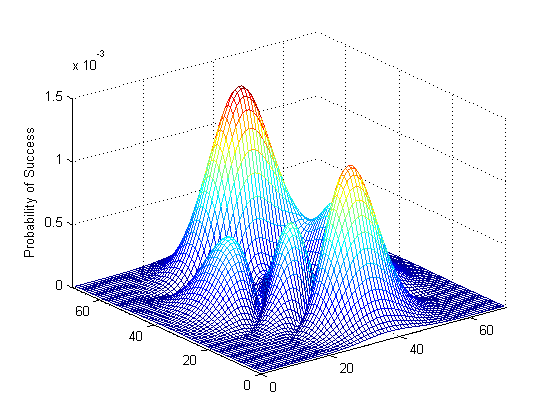
\includegraphics[scale=0.5]{../Matlab/Images/InitialProbDist.png}
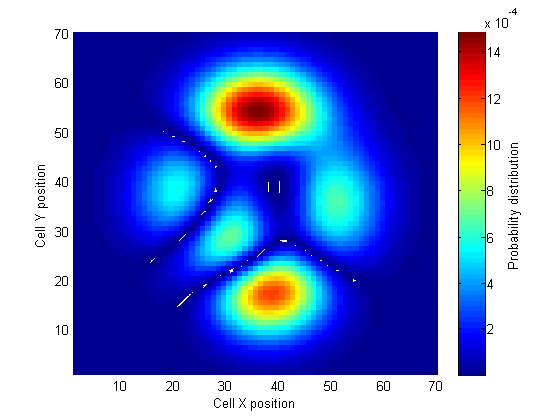
\includegraphics[scale=0.5]{../Matlab/Images/InitialProbDistSurf.png}
\caption{Probability distribution used in Monte Carlo simulation}
\end{center}\end{figure}

It is worth noting that a grid resolution of 70 was chosen. As computation time increases with the square of grid size, a sufficiently low value was chosen for computation which simultaneously allowed for sufficiently high resolution. 

Additionally, the model is invariant under cell size. Each search iteration is not represented in the time used to search a cell, so the total work done in searching a cell is ``one unit.'' The conversion from the single unit work to time changes based on cell size, but is not modeled.

Initial allocation was then performed on the ships in this distribution. This placed the $n$ ships in the grid according to the highest $\epsilon$ values. The probability distribution is then evolved assuming failure of search. 

\begin{figure}[H]\begin{center}
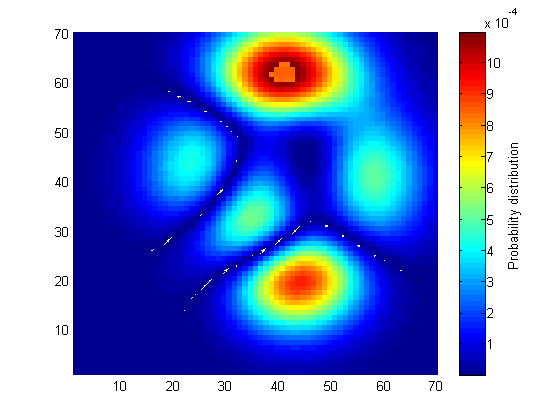
\includegraphics[scale=0.35]{../Matlab/Images/ModelSearch001.png}
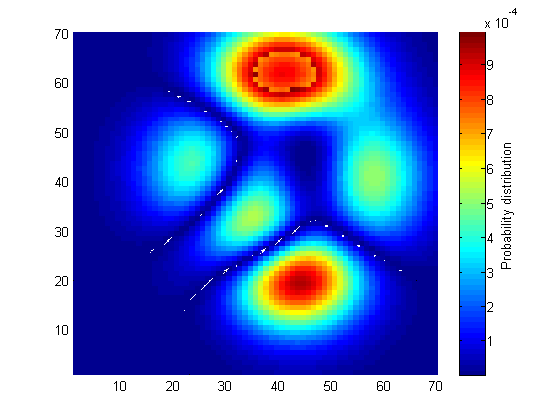
\includegraphics[scale=0.35]{../Matlab/Images/ModelSearch020.png}
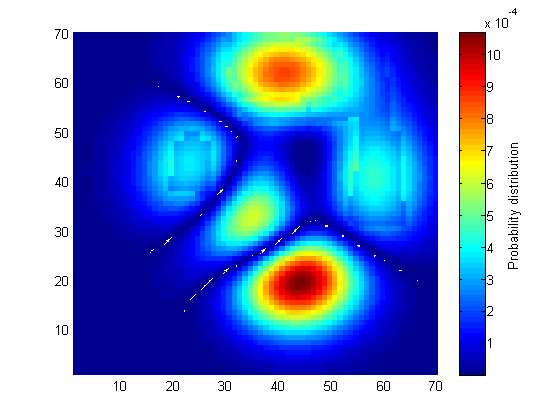
\includegraphics[scale=0.35]{../Matlab/Images/ModelSearch100.png}
\caption{Prob. dist. of 15 ships after 1, 20, and 100 search iterations respectively.}
\end{center}\end{figure}

As can be seen, the probability of the object's presence in unsearched squares increases, and the probability in searched squares decreases. 

The technology is considered to be functionally uniform. As is noted in section 2.2, the effectiveness of searching a square drops with the number of times the square has been searched. This is intuitively correct; because the square has been searched before, it is less likely to be successfully searched on the second iteration. As a consequence, $\beta$ decreases with search count. This can be seen in figure 4.

\begin{figure}[H]\begin{center}
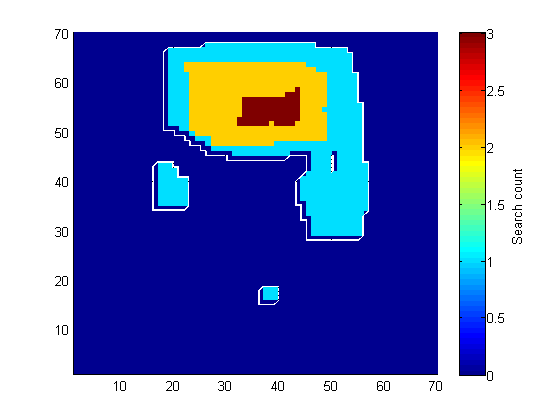
\includegraphics[scale=0.5]{../Matlab/Images/After100SearchCount.png}
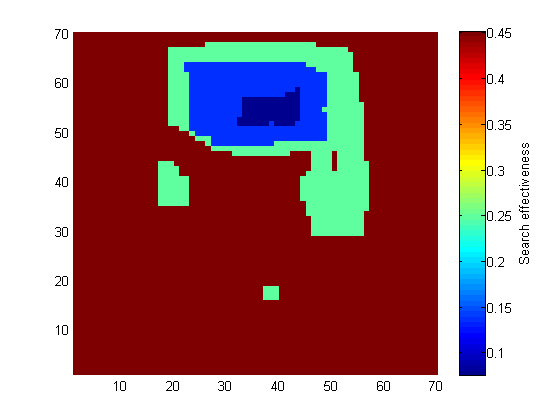
\includegraphics[scale=0.5]{../Matlab/Images/After100SearchEffectiveness.png}
\caption{Search count map (left) and $\beta$ values map (right) after 100 iterations with 15 ships. Note that $\beta$ values decrease where searches have already happened.}
\end{center}\end{figure}

\subsection{Cost function analysis}

The cost function as written above may appear arbitrary. To some extent, it is. However, it is effective at serving its purpose: to minimize the distance traveled by the ships with respect to the effectiveness of the overall search. In order to determine whether this cost functions serves its purpose well, two functions were compared. The first, $\gamma_{t1}(j,k)=1$, disregards distance traveled. The second, $\gamma_{t2}(j,k)=d_{\mbox{traveled}}$ uses the distance as a cost. What follows is an evolution of the two cost functions.

\begin{figure}[H]\begin{center}
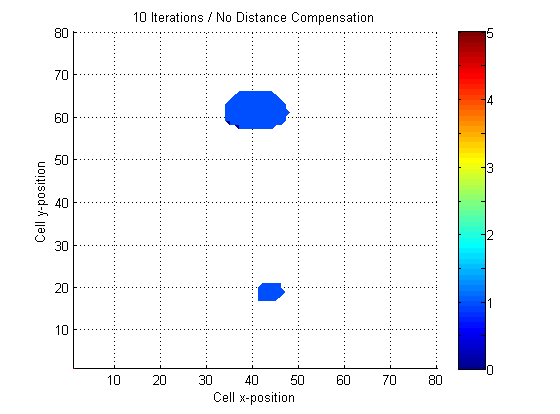
\includegraphics[scale=0.45]{../Matlab/Images/SearchCountNoDist010.png}
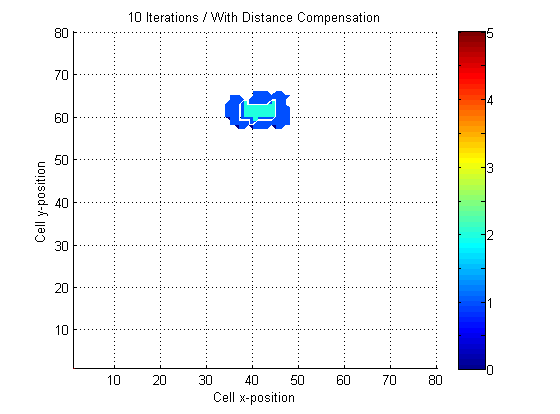
\includegraphics[scale=0.45]{../Matlab/Images/SearchCountDist010.png}
\caption{Evolution comparison at 10 iterations}
\end{center}\end{figure}

After 10 iterations, the difference between $\gamma=1$ and $\gamma=d$ is apparent. In $\gamma=1$, ships have appeared and have searched in the lower portion of the search space. However, in $\gamma=d$, ships have remained near the first local maximum, frequently searching twice rather than moving somewhere else.

\begin{figure}[H]\begin{center}
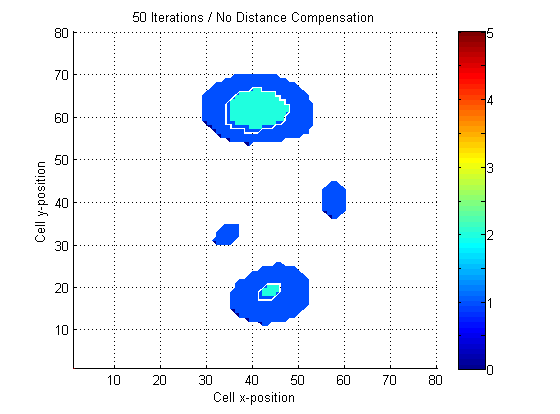
\includegraphics[scale=0.45]{../Matlab/Images/SearchCountNoDist050.png}
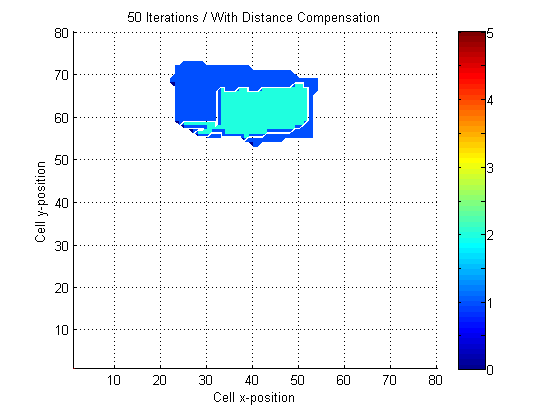
\includegraphics[scale=0.45]{../Matlab/Images/SearchCountDist050.png}
\caption{Evolution comparison at 50 iterations}
\end{center}\end{figure}

After 50 iterations, $\gamma=1$ has evolved to the point where the lower maximum has been searched twice. This is the lowest search iteration (rounded to the nearest 10) for which this is true. By comparison, the $\gamma=d$ search regime has searched the upper maximum and surrounding area extensively, but has not moved from there. The next notable point occurs at 230 iterations.

\begin{figure}[H]\begin{center}
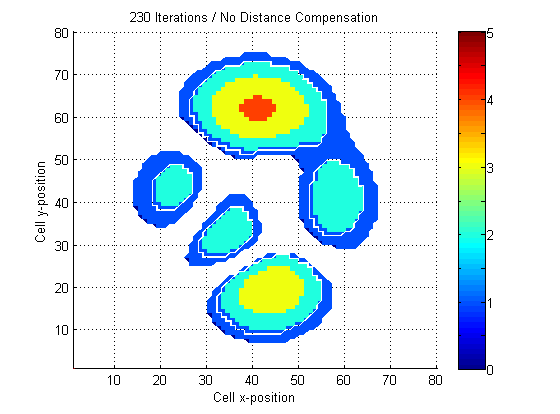
\includegraphics[scale=0.45]{../Matlab/Images/SearchCountNoDist230.png}
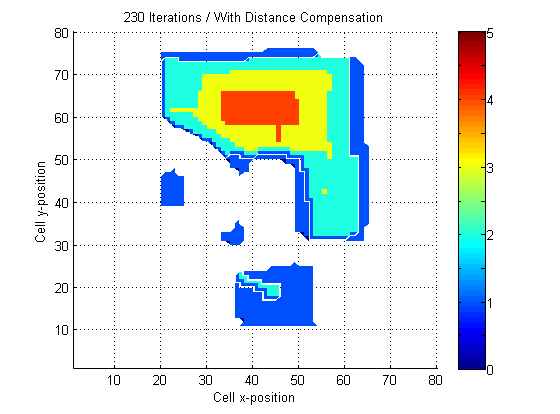
\includegraphics[scale=0.45]{../Matlab/Images/SearchCountDist230.png}
\caption{Evolution comparison at 230 iterations}
\end{center}\end{figure}

At 230 iterations, the $\gamma=d$ search regime has begun to scan the lower maximum. This is in contrast to the $\gamma=1$ regime, which has scanned the lower maximum significantly more thoroughly.

The progression of the $\gamma=1$ regime matches the local maxima of the base probability in figure 2. Because $\gamma=1$, the value of $\epsilon$ merely follows: $$\epsilon = p(j)*\beta(j,k)$$

Search vessels simply move to the places where the probability of discovering something is highest. This, naturally, roughly follows the original distribution map.

\subsection{Effect of the $\gamma=d$ search regime}

The $\gamma=d$ search regime does not leave its localized area until approximately five times later than the $\gamma=1$ regime. This is potentially unwanted behavior. 

However, this is not the complete picture. To understand the significant role the cost function plays in the optimization process, one must look at the total distance traveled by ships:

\begin{figure}[H]\begin{center}
\begin{tabular}{|c|c|c|}
\hline & $DT$ & $PD$\\\hline\hline
$\gamma=1$ & 144902 & $45.7\%$\\\hline
$\gamma=d$ & 3809 & $43.8\%$\\\hline
\end{tabular}
\caption{DT: Distance Traveled (cells); PD: Probability of Discovery}
\end{center}\end{figure}

The difference here is profound. Without optimizing for distance, the distance the ships travel is $\approx 38$ times that of $\gamma=d$. The gain in effectiveness is only $1.9\%$. Therefore, by sacrificing roughly two percent of our distance movement, we gain a 38-fold reduction in distance traveled.

\subsection{Sensitivity analysis of $PD$}

One of the most critical components of the model is the probability that the search has discovered the object. It is important to understand how this probability varies with the model inputs. In order to evaluate this, the data from the Monte Carlo simulation was passed through a logarithmic fit.

\begin{figure}[H]\begin{center}
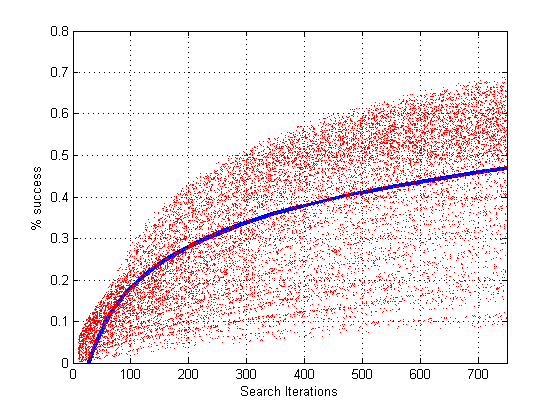
\includegraphics[scale=0.5]{../Matlab/Images/LogSearchIterPctSuccessMSE0.png}
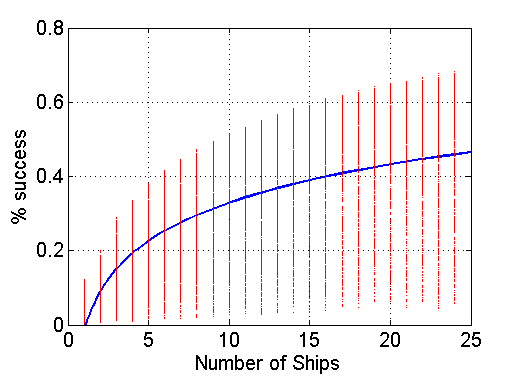
\includegraphics[scale=0.5]{../Matlab/Images/LogShipCtPctSuccessMSE0.png}
\caption{Log fit lines in blue; Search iter fit line: $-0.4809+0.3304*log_{10}(x)$; Ship iter fit line: $-0.0142+0.3433*log_{10}(x)$}
\end{center}\end{figure}

Two notes about these graphs: first, the number of ships is a discrete quantity between 1 and 25. The number of search iterations is discrete as well, though fine enough to appear continuous. Second, the mean squared error on both graphs is $< 0.02$.

It is clear that the percent success provides diminishing returns as iteration count increases, and as number of ships increases. The limiting factor here is the $\beta$ function - as the total number of searches goes up, the returns decrease on the whole.

Combined, these two form the primary distribution indicating the success of the search:

\begin{figure}[H]\begin{center}
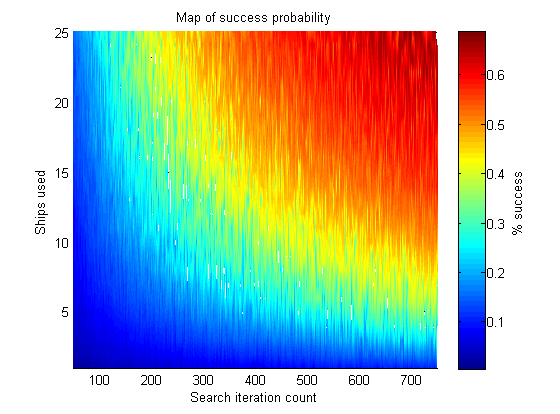
\includegraphics[scale=0.75]{../Matlab/Images/PctSuccessByItersShips.png}
\caption{Histogram of the probability of success. Vertical noise is a result of interpolation.}
\end{center}\end{figure}

This histogram suggests that the contour lines of the probability success graph are of the form $\frac 1x$. Additionally, this map shows that the net probability is likely of the form $\log(n*i)$, where $n$ is the number of ships used and $i$ is the number of iterations performed (as in Figure 1).

The coefficients of the logarithmic fits suggest that this is true: the coefficient with respect to ships used is $0.3433$, and the coef. with respect to iterations is $0.3304$. This is a $3.76\%$ difference. The only significant difference lies in the intercept of the functions. However, the growth rate of the functions is the same.

This makes intuitive sense. The total number of searches is equal to $n*i$, and a relatively logarithmic limit is expected. While the distribution must taper off to $1$, and cannot proceed to $\infty$, it is locally logarithmic.

\subsection{Sensitivity of Distance Traveled}

The distance traveled is revealed to be linear with respect to the number of ships and number of iterations. These results both confirm what one might intuitively surmise: each iteration will have an approximately constant travel distance, and each ship will travel the same distance in an iteration.

The following comparisons were extracted from the Monte Carlo simulation:

\begin{figure}[H]\begin{center}
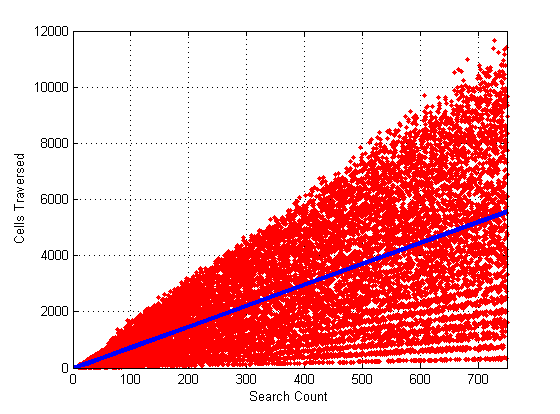
\includegraphics[scale=0.5]{../Matlab/Images/DistTraveledByIterCount.png}
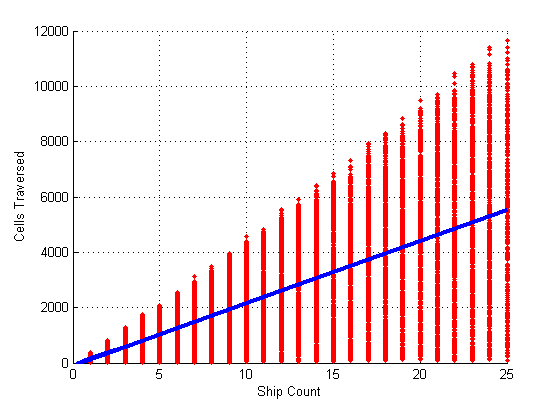
\includegraphics[scale=0.5]{../Matlab/Images/DistTraveledByShipCount.png}
\caption{Blue lines are linear fits; Search count linear fit: $7.4547x-26.2551$; ship count linear fit: $223.9765x-88.9555$.}
\end{center}\end{figure}

This suggests that the distance traveled (and, in theory, at least part of the cost of searching) increases linearly with both distance and search count. 

The reason this holds some significance is that one might expect the distance traveled to grow over time, since the nearby probabilities are diminished, but in reality, this is not the case.

\subsection{Sensitivity of Computation Time}

\begin{figure}[H]\begin{center}
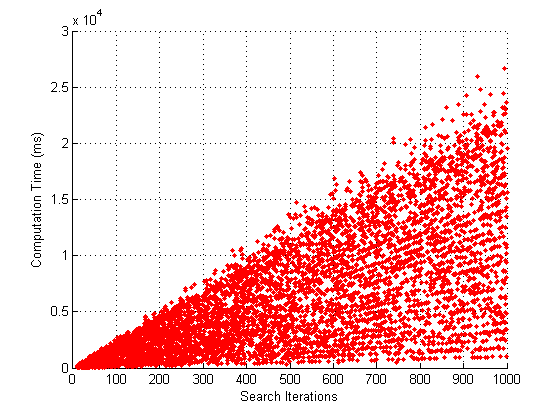
\includegraphics[scale=0.48]{../Matlab/Images/CompTimevsSearchIterations.png}
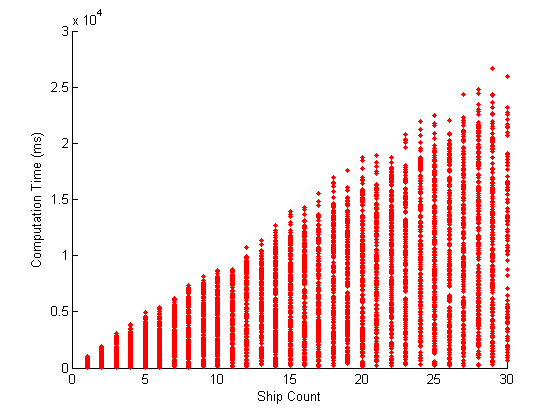
\includegraphics[scale=0.48]{../Matlab/Images/CompTimevsShipCount.png}
\caption{Showing the computation time is linear in both search iterations and ship count}
\end{center}\end{figure}

The computation time is visibly linear with respect to search iterations and ship count. While time is included in milliseconds, and individual milliseconds are not reproducible, the rate of growth is constant. 

\begin{figure}[H]\begin{center}
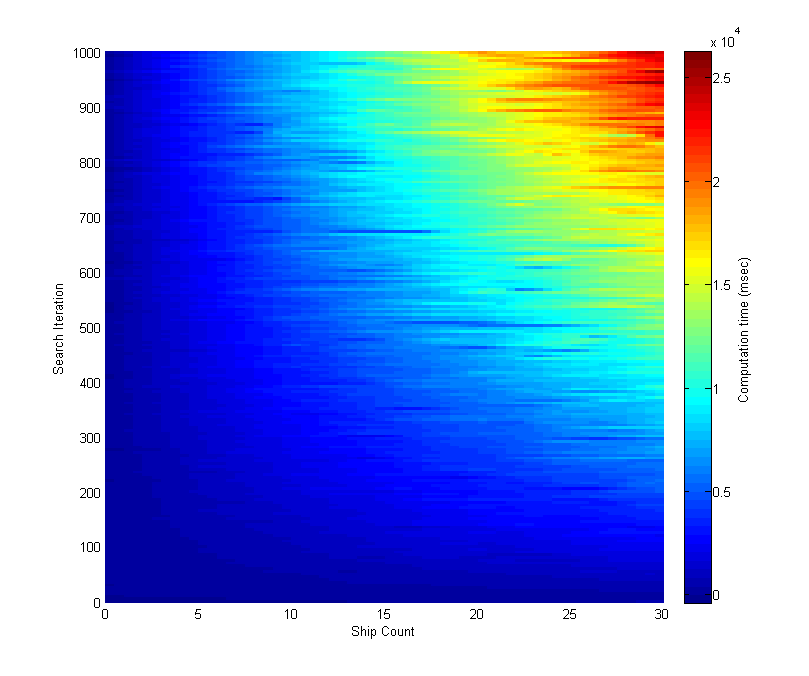
\includegraphics[scale=0.7]{../Matlab/Images/CompTimeByItersShips.png}
\caption{Shows computation time as linear with respect to iteration count.}
\end{center}\end{figure}

This implies that the model operates in $O(n*i)$, where $n$ is the number of vessels and $i$ is the number of iterations.

\subsection{Anomalous behavior of $\alpha$ values}

The sensitivity of $\alpha$ has been deferred to this section because its behavior is highly anomalous in comparison to the other model behaviors. A summary of the results of $\alpha$ are included here. Specific dynamics of $\alpha$ are not investigated in this paper.

The first dynamic to highlight is the odd independence of $\alpha$ on $PD$, shown in figure 14. The distribution of $PD$ over $\alpha$ appears to be relatively uniform; however, there is visibly higher density toward the bottom left and upper right. Additionally, there is an odd behavior pattern wherein the success rate seems to fall off once $\alpha$ grows sufficiently large. 

\begin{figure}[H]\begin{center}
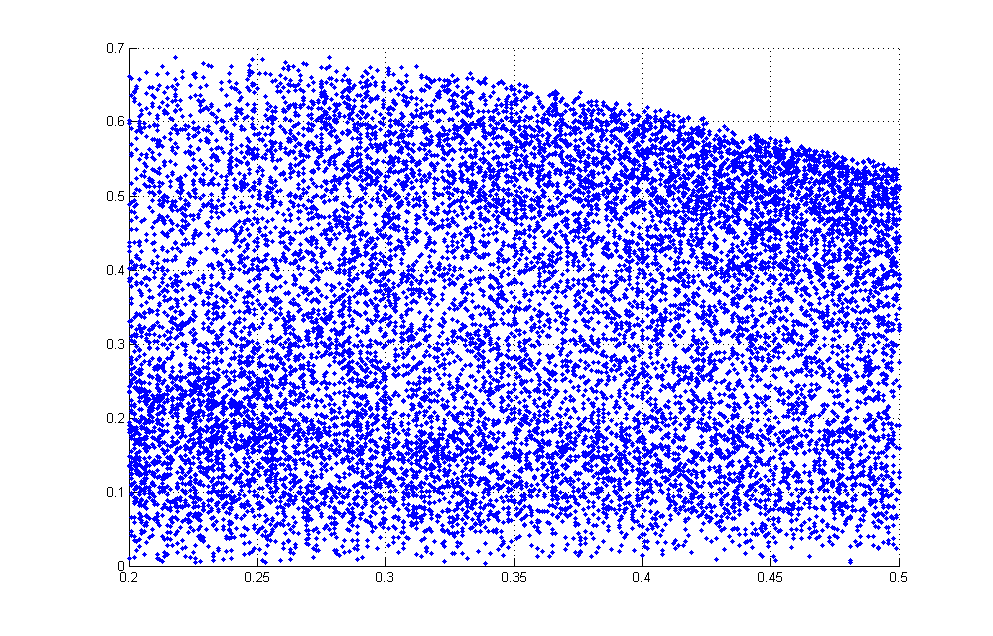
\includegraphics[scale=0.3]{../Matlab/Images/PctSuccessByAlpha.png}
\caption{Distribution of $\alpha$ versus the percent success rate}
\end{center}\end{figure}

In order to investigate this behavior further, a moving average was taken of $\alpha$ verses $PD$:

\begin{figure}[H]\begin{center}
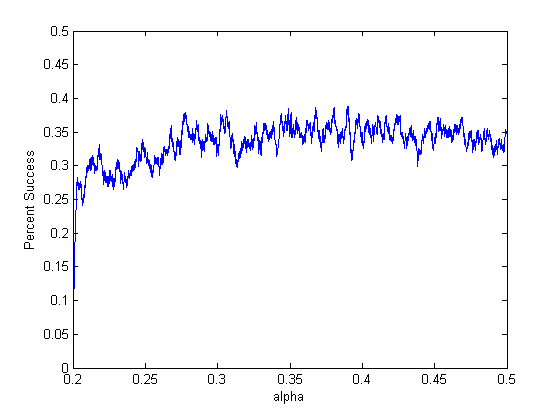
\includegraphics[scale=.5]{../Matlab/Images/MovAvgAlphaPctSuccess.png}
\caption{A moving average of $\alpha$ versus the percent rate with smoothing 100 (over 15000 data points).}
\end{center}\end{figure}

This seems to indicate that, for an $\alpha$ around 0.28, the search success does not suffer, but it seems to begin to suffer slightly past another $\alpha$ around 0.43. However, this is a purely qualitative assessment, and does not represent any statistical measurement.

Nevertheless, $\alpha$ is sufficiently linear over the operating range of values that the dynamics of this value may not impact the model in operation; it is strictly a mathematical exercise.

\section{Future studies}

There are several areas of future study. The first is, of course, $\alpha$ dynamics. It is necessary to understand how the $\alpha$ value impacts the model. For now, however, it is sufficient to assume that the $\alpha$ value does not have a considerable impact on the net search outcome. 

Additionally, there is one chart which has a yet-unexplained anomaly in figure 16:

\begin{figure}[H]\begin{center}
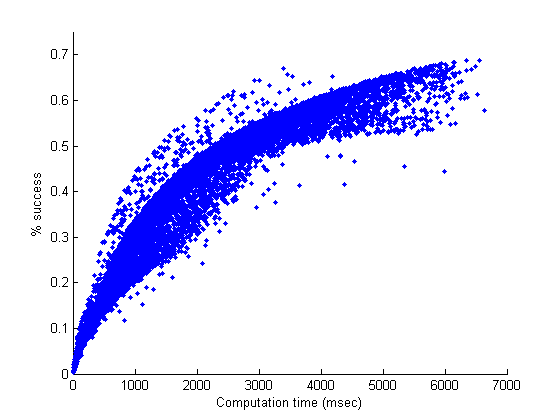
\includegraphics[scale=0.75]{../Matlab/Images/CompTimePctSuccess.png}
\caption{Odd dynamics exhibited by computational time and percent success}
\end{center}\end{figure}

The computational time follows a strongly logarithmic plot in the normal case, but there are two locations where this does not hold. The first set of points appears above the obvious logarithmic boundary (which is not currently characterized). These points may very well be computational anomalies, but it is worth investigating to see whether they are truly anomalous or if they are indicative of a better-than-average case. There is a chance - albeit a small one - that they \textit{do} represent a better-than-average case that can be characterized. 

Additionally, a second unexplained behavior occurs around 3000 msec. The underside of the graph begins to expand outward - but it suddenly converges again in with the main path around 3000 msec. The cause of this is unknown, and this behavior is as yet uncharacterized. 

Finally, additional probability distributions would need to be studied in order to reach a definitive conclusion about the model dynamics.

\pagebreak

\begin{thebibliography}{10}
\bibitem{TF} T. Furukawa, F. Bourgault, B. Lavis, H.F. Durrant-Whyte, \emph{``Recursive Bayesian Search-and-Tracking Using Coordinated UAVs for Lost Targets"}, IEEE International Conference on Robotics and Automation, 2006. 

\bibitem{JA} \emph{``Search for MH370 Facts and statistics Surface search of the southern Indian Ocean 17 March–28 April 2014"}, Joint Agency Coordination Centre, http://www.jacc.gov.au/search/files/MH370_Facts_and_statistics-Surface_search_of_the_southern_Indian_Ocean, PDF.

\bibitem{LL} L.C.M. Lebreton, S.D. Greer, J.C. Borrero, \emph{``Numerical modeling of floating debris in the world’s oceans"}, Marine Pollution Bulletin, Volume 64, Issue 3, March 2012, Pages 653-661, ISSN 0025-326X, http://dx.doi.org/10.1016/j.marpolbul.2011.10.027.

\bibitem{Mackay98} D.J.C. Mackay, \emph{``Introduction to Monte Carlo Methods"}, submitted for publication.

\bibitem{HR} Henry R. Richardson and Lawrence D. Stone, \emph{``Operations analysis during the underwater search for Scorpion"}, submitted for publication. 

\bibitem{Stone75} Lawrence D. Stone, \textit{Theory of Optimal Search}, New York: Academic Press, 1975.

\bibitem{LS} Lawrence D. Stone, Colleen M. Keller, Thomas M. Kratzke, Johan P. Strumpfer, \emph{``Search for the Wreckage of Air France Flight AF 447"}, Statistical Science 2014, Vol. 29, No. 1, 2014.
\end{thebibliography}

\end{document}